\begin{problem}{Life is short.So just eat!}{standard input}{standard output}{0.5 second}{512 megabytes}

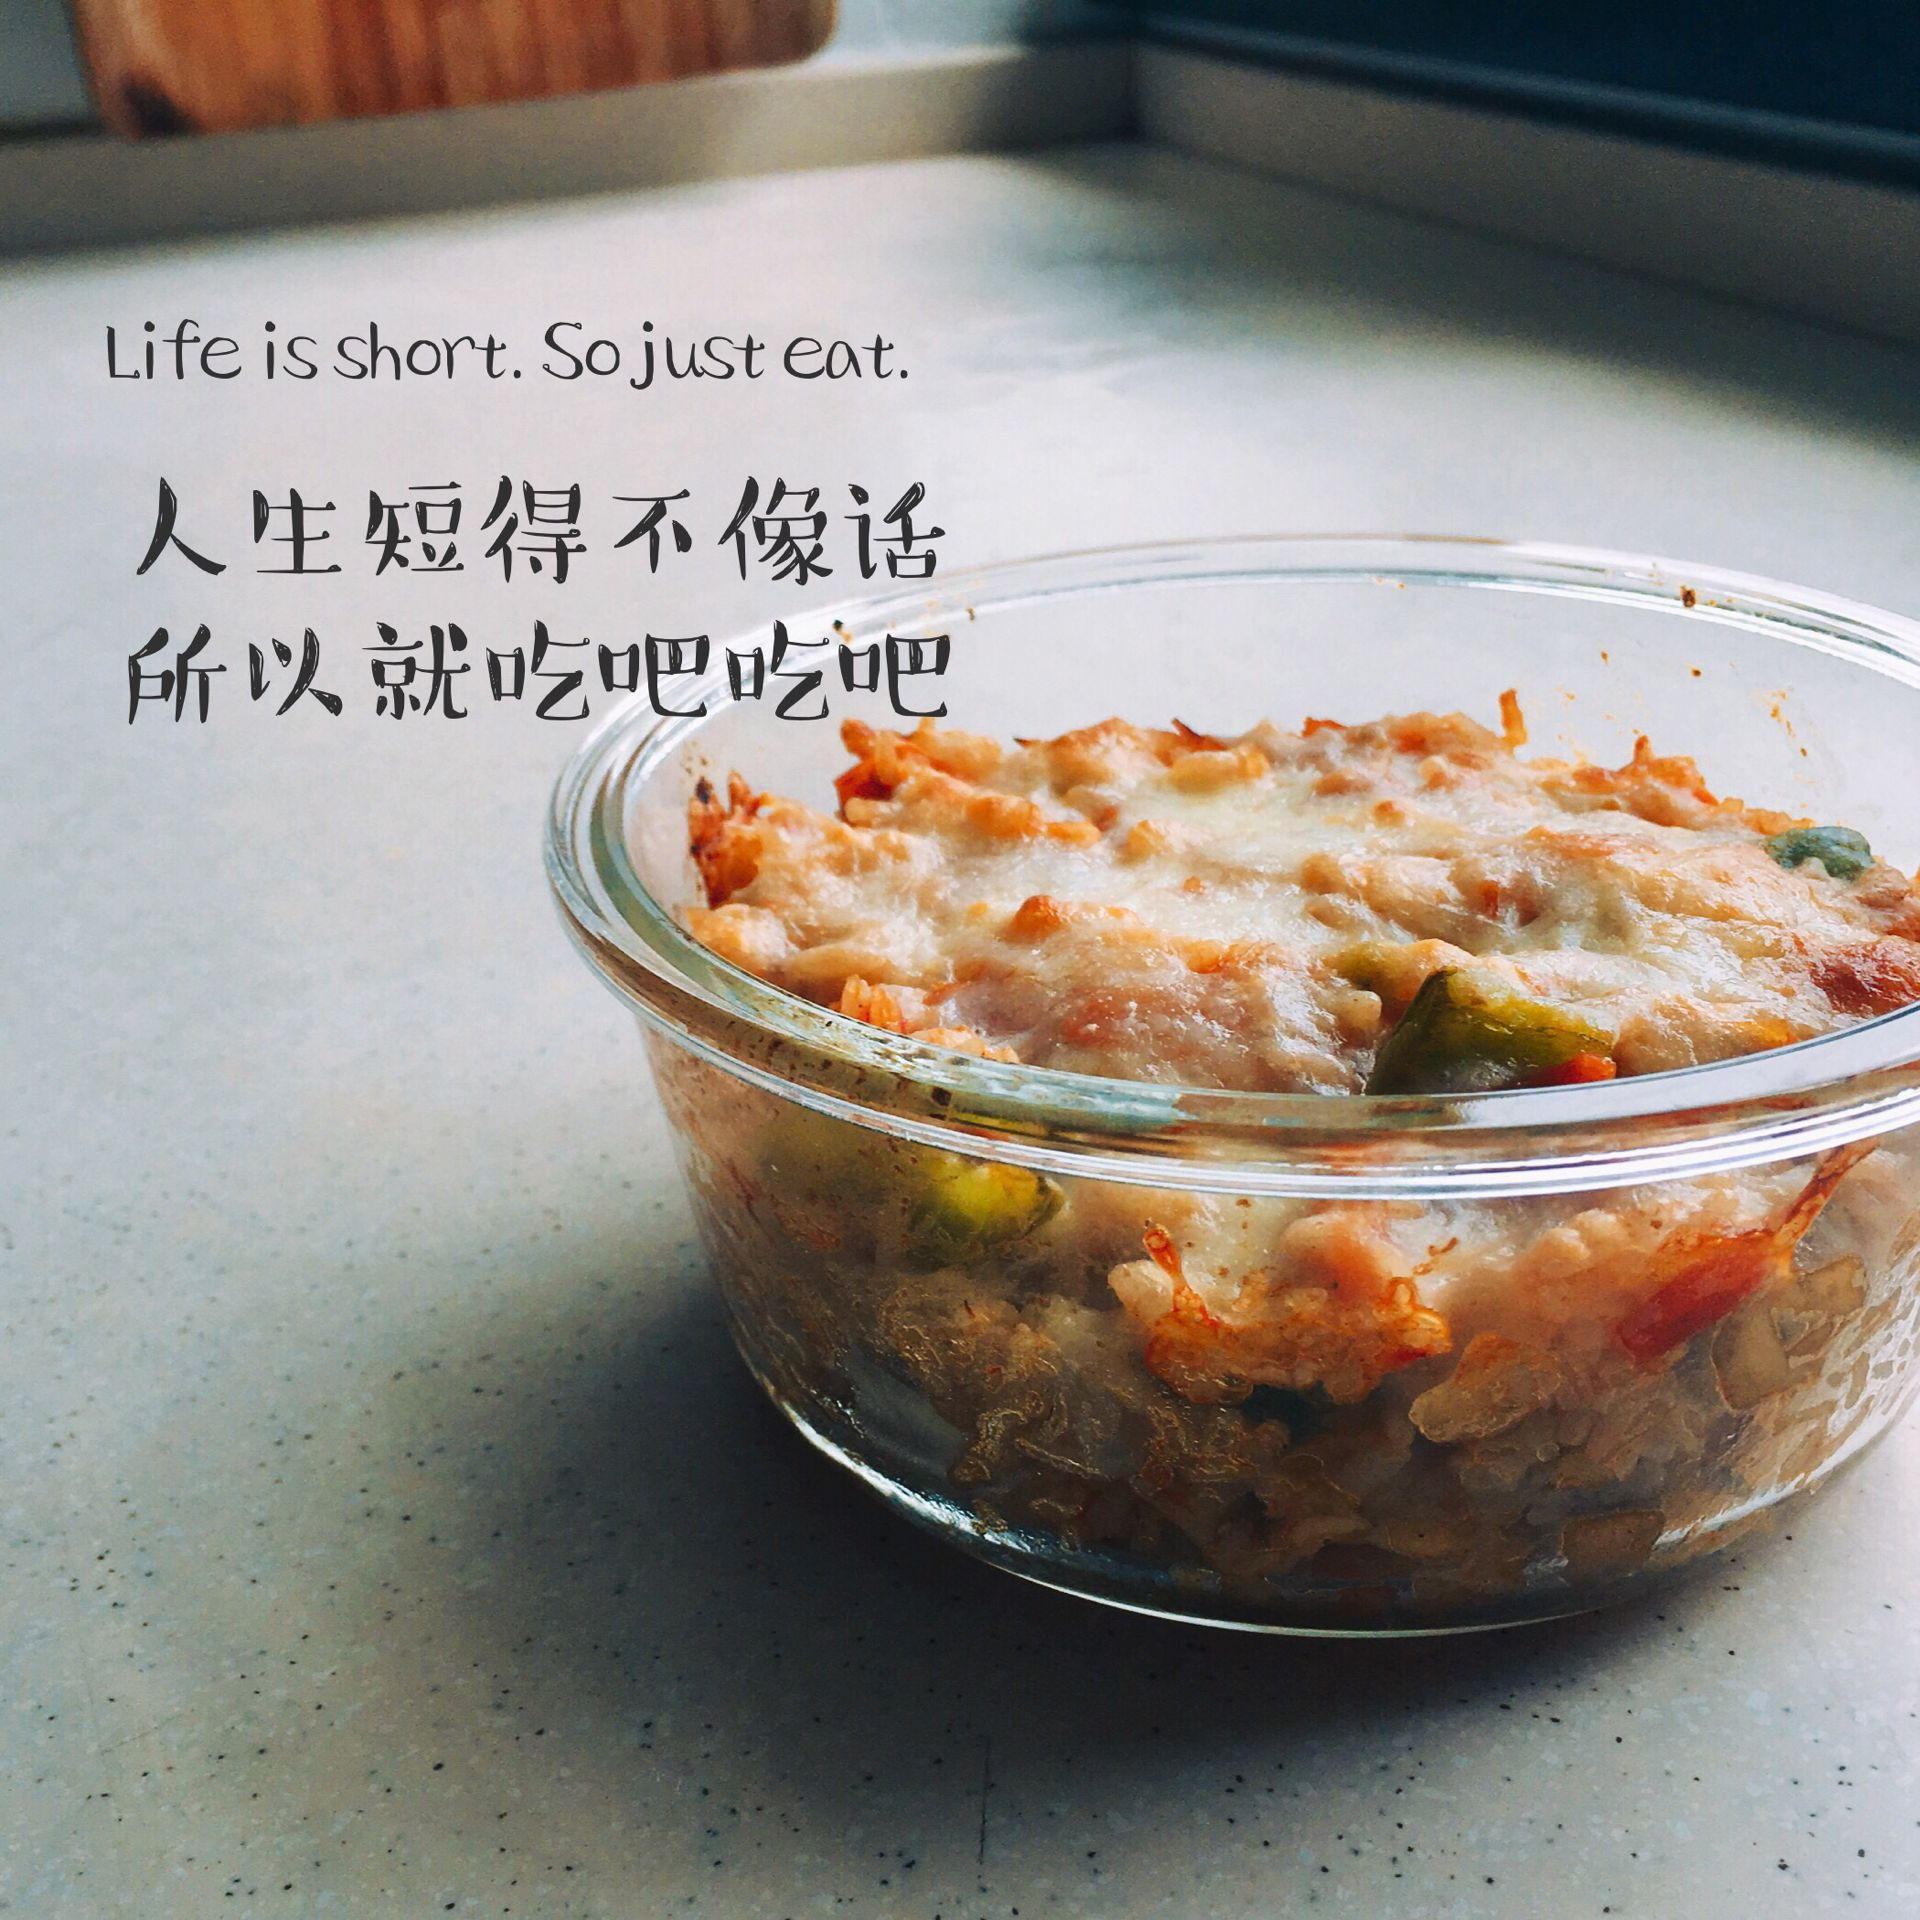
\includegraphics[width=0.60\textwidth]{ak.jpg}%

Life is short. So just eat!

Zhuangba 十分热爱生活,对待吃的毫不马虎。

有一天, rkmdsxmds 和 Zhuangba 一起在美食城吃美食。美食城有 $n$ 家店,这其中有 $n-1$ 条道路使得美食城中的每家店都联通。每家店做的美食有 $d_i$ 的美味值。其中 $1$ 号店是日料店, Zhuangba 最喜欢吃日料了!

现在, rkmdsxmds 和 Zhuangba 有 $q$ 个计划,每次美食行程为从 $u$ 号店前往 $v$ 号店(走最短路径),数据保证 $v$ 在 $u$ 前往日料店的最短路径上。

每次美食行程开始时,Zhuangba 手上有为美味值为 $w$ 的美食,并且每当经过某家店时(包括 $u$ 和 $v$),假如那家店的美食比 $Zhuangba$ 所有已有美食美味值更高(严格大于),那么 $Zhuangba$ 就会买买买(记作一次购买事件)!

现在 $rkmdsxmds$ 想知道每一次美食行程,会进行多少次购买事件。

\InputFile
第一行,两个正整数$n , q。(2\le n \le 10^{5}, 1\le q \le 10^{5})$ 。

第二行,$n$ 个正整数 $d_i(1\le d_i \le 10^5)$ 描述每家店售卖美食的美味值。

接下来 $n-1$ 行,每行描述一条道路 $x, y(1\le x, y \le n)$,表示有一条$x$ 和 $y$ 之间有道路。

接下来 $q$ 行,每行描述一次美食行程 $u , v , w(1\le u,v \le 10^5, 1 \le w \le 10^5)$。

\OutputFile

输出 $q$ 行,第 $i$ 行表示第 $i$ 次美食行程中的购买事件。 

\Example

\begin{example}
\exmpfile{example.1.in}{example.1.ans}%
\end{example}

\end{problem}
